\documentclass[12pt]{article}

\usepackage{sbc-template}
\usepackage{graphicx,url}
\usepackage[brazil]{babel}
\usepackage[utf8]{inputenc}   % UTF-8 encoding is recommended by ShareLaTex
\usepackage[T1]{fontenc}      % possibilita copiar textos com acentos.

\sloppy

\title{A Formação de Professores de Matemática Voltada para a Prática com Alunos com Deficiência Visual: Revisão Sistemática}

\author{Pedro Lealdino Filho\inst{1}\inst{2}, Autor 2\inst{1}, Sani Rutz de Carvalho\inst{1}}

\address{Programa de Pós-Graduação em Ensino de Ciência e Tecnologia \\ 
Universidade Tecnológica Federal do Paraná \\
  Ponta Grossa -- Paraná -- Brasil.
  \nextinstitute
     Institut de Recherche sur l'Enseignement des Mathématiques (IREM) \\
    Université Claude Bernard - Sciences, Société, Historicité, Éducation et Pratiques (S2HEP) \\
    Villeurbanne -- Lyon -- France
  \email{pedro.lealdino@etu.univ-lyon1.fr  }
}

\begin{document}

\maketitle

\begin{abstract}
In this study, we aim to investigate the didactic-pedagogical interventions in Mathematics Teacher Training regarding the teaching of mathematics to students with visual impairment. We used a systematic descriptive review of the literature contained in articles, available in the Scopus, Google Scholar and Scielo databases from 1994 to 2019. We used the descriptors: xxx, xxx, xxx, and located 538 searches. After selection, we considered 12 studies as the final review sample. We can infer that the studies present a great geographical diversification, but as a predominance for the English language in the articles. ... We have seen advances in the field of teaching mathematics for the blind, but the volume of this type of study is still small. We stress the need for further research that meets and highlights the difficulties of training graduate professionals in mathematics in practice with visually impaired students to perform a more inclusive and effective education in public educational environments.
\end{abstract}

\begin{resumo}
Neste estudo objetivamos investigar as intervenções didático-pedagógicas na Formação de Professores de Matemática com relação ao ensino de matemática a alunos com deficiência visual. Utilizamos uma revisão sistemática descritiva da literatura contida em artigos, disponíveis nas bases de dados Scopus, Google Scholar e Scielo nos anos de 1994 a 2019. Utilizamos os descitores: xxx, xxx, xxx, e localizamos 538 pesquisas. Após a seleção, consideramos 12 estudos como amostra final da revisão. Podemos inferir que os estudos apresentam uma diversificação geográfica grande, mas como uma predominância para a língua inglesa nos artigos. ... . Observamos avanços na área do ensino de matemática para cegos, mas o volume desse tipo de estudo ainda é pouco. Salientamos a necessidade da realização de mais pesquisas que, atendam e evidenciem as dificuldades da formação dos profissionais licenciados em matemática na prática com alunos com deficiência visual para execução de uma educação mais inclusiva e efetiva em ambientes educacionais públicos. 

\end{resumo}

\section{Introdução}

Ensinar matemática é um desafio. Tem sido um desafio e podemos concluir isso pelos inúmeros esforços de diversas equipes de pesquisa do mundo inteiro empenhados em facilitar o processo de ensino e aprendizagem de matemática. Grandes comitês e eventos internacionais tais como Congressos, Seminários, Mesas redondas acontecem todos os anos com o mesmo objetivo: Fazer com que a matemática seja ensinada de forma efetiva para todos.


\subsection{Como se forma um professor de matemática no Brasil?}
Conforme o parecer CNE/CES 1.302/2001 homologado e publicado no Diário Oficial da União de 5/3/2002, Seção 1, p. 15, os cursos de Licenciatura em Matemática tem por objetivo principal a formação de professores para a educação básica. Neste documento, há uma ênfase nas habilidades e competências que o acadêmico deve adquirir no processo formativo tais como o raciocínio lógico, a postura crítica, a capacidade de resolver problemas, de analisar, selecionar e produzir materiais didáticos, desenvolver estratégias de ensino que favoreçam a criatividade, a autonomia e a flexibilidade do pensamento matemático dos educandos, buscando trabalhar com mais ênfase nos conceitos do que nas técnicas, fórmulas e algoritmos. \cite{leite2009formaccao}

\noindent
Nesse sentido, a formação dos professores deve atender às necessidades e aos desafios da atualidade. Para tanto, \cite{pletsch2009formaccao} sugere que o professor seja formado de maneira, a saber, mobilizar seus conhecimentos, articulando-os com suas competências mediante ação e reflexão teórico-prática. 

\noindent
A Proposta de Diretrizes para a Formação de Professores da Educação Básica delineia as exigências que se colocam para o desempenho do papel docente frente às novas concepções de educação no mundo contemporâneo:

\begin{quote}
    Orientar e mediar o ensino para a aprendizagem dos alunos; responsabilizar-se pelo sucesso da aprendizagem dos alunos; assumir e saber lidar com a diversidade existente entre os alunos; incentivar atividades de enriquecimento curricular; elaborar e executar projetos para desenvolver conteúdos curriculares; utilizar novas metodologias, estratégias e material de apoio; desenvolver hábitos de colaboração e trabalho em equipe. \cite{mec2000}
\end{quote}

\noindent
Inúmeros são os estudos que reafirmam a necessidade da melhoria da formação de professores como condição essencial e premente para a promoção eficaz da inclusão com necessidades especiais em rede regular de ensino \cite{pletsch2009formaccao}, \cite{bueno1999crianccas}, \cite{antunes2011formaccao}, \cite{antuneseducaccao}, \cite{glat2004papel}, \cite{magalhaes1999viver}. A realidade evidenciada por uma pesquisa de \cite{ferreira20031} mostrou que os professores, de maneira geral, não estão preparados para receber em sua sala de aula alunos especiais. 

\noindent
Quanto ao corpo curricular em licenciatura em matemática, o parecer \cite{diretrizesmatematica2001} instrui que os conteúdos, comuns a todos os cursos de Licenciatura, podem ser distribuídos ao longo do curso de acordo com o currículo proposto pela IES:
\begin{itemize}
    \item Cálculo Diferencial e Integral
    \item Álgebra Linear
    \item Fundamentos de Análise
    \item Fundamentos de Álgebra
    \item Fundamentos de Geometria
    \item Geometria Análitica
\end{itemize}
\noindent
O parecer ainda instrui que, a parte comum deve incluir:
\begin{itemize}
    \item conteúdos matemáticos presentes na educação básica nas áreas de Álgebra, Geometria e Análise;
    \item conteúdos de áreas afins à Matemática, que são fontes originadoras de problemas e campos de aplicação de suas teorias;
    \item conteúdos da Ciência da Educação, da História e Filosofia das Ciências e da Matemática.
\end{itemize}

\noindent
Diante disso, a especificidade da educação inclusiva em matemática se torna vaga, deixando a critério de cada IES incentivar a formação de professores para a inclusão. Com isso, como afirma \cite{pletsch2009formaccao}, perdem os educandos, os educadores e toda a sociedade, pois a profissão docente precisa dar respostas adequadas e fazer as necessárias intervenções que envolvem situações diversas e singulares do desenvolvimento humano.

\section{Metodologia}

Uma revisão sistemática é um meio de identificar, avaliar e interpretar todo o corpo de pesquisas disponíveis relevantes a um tópico de pesquisa particular, questões de pesquisa, ou fenômeno de interesse \cite{kitchenham2004procedures}. Boas revisões sistemáticas tomam precauções importantes para minimizar erros e conclusões tendenciosas \cite{littell2008systematic}.

\noindent
Para realizar a revisão sistemática apresentada neste estudo, um plano detalhado foi desenvolvido, baseando-nos em pesquisas correlatas (\cite{da2018processo}) utilizando sete etapas: construção do protocolo, definição da pergunta, busca dos estudos, seleção dos estudos, avaliação crítica, coleta dos dados e síntese dos dados \cite{galvao2009revisao}, descritas a seguir:
\begin{itemize}
    \item \textit{Construção do Protocolo}: fase de planejamento da revisão sistemática, em que definimos a pergunta, as bases de pesquisa, os critérios de seleção dos estudos, os procedimentos de busca, a avaliação e a análise dos estudos;
    \item \textit{Definição da Pergunta}: como base para o estudo, nos orientamos pela pergunta inicial: "Quais intervenções didático-pedagógicas têm sido utilizadas na Formação de Professores para o ensino de matemática aos alunos cegos?" 
    \item \textit{Busca dos Estudos:} este trabalho utilizou-se das bases: Google Scholar, Scopus, Springer e Scielo foi realizada para identificar pesquisas empíricas, publicadas entre janeiro de 1994 e outubro de 2019, que tinham como objeto a formação de professores de matemática na prática com alunos deficientes visuais. A pesquisa incluiu os seguintes descritores: Formação de professores, Formação em Serviço, Deficiência Visual, Cegos, Matemática, Pesquisa Empírica. Tais descritores serviram como um filtro mais largo de pesquisa. Para as palavras-chave, foram estabelecidas as seguintes: Matemática, Professores, Deficiência Visual. 
    \item \textit{Seleção dos Estudos}: Os critérios de inclusão foram: 1) A amostra de cada estudo incluia exclusivamente professores de alunos com algum tipo de deficiência visual; 2) Os estudos tinham como objetivo avaliar, empiricamente, as práticas pedagógicas dos professores; 3) Os artigos deveriam ser publicados em revista. Dados demográficos, o tamanho da amostra e os instrumentos de diagnóstico foram abstraídos. 
    As buscas foram limitadas a artigos publicados entre 1994 e 2019 levando-nos a encontrar um total de 538 trabalhos. Depois de examinar os títulos e a lista de referências para buscar trabalhos correlatos, ficamos com um total de 28 pesquisas. Após lermos cada um desses artigos, excluímos 16 outros por não atenderem os critérios definidos. Assim, obtivemos um total de 12 artigos para análise detalhada. Fig \ref{fig:revisao_sistematica_fluxograma}.
    \item \textit{Avaliação Crítica:} A avaliação crítica dos estudos foi realizada conforme o objetivo central da revisão, analisando as intervenções didático-pedagógicas na Formação de Professores de matemática na prática com alunos deficientes visuais nos últimos 25 anos. Este período foi definido pelo início da Declaração de Salamanca, em 1994. 
    \item \textit{Coleta de Dados:} Encontramos 538 trabalhos entre artigos. Depois de salvos, iniciamos o procedimento de seleção da amostra da revisão sistemática. 
    \item \textit{Síntese dos Dados:} Trata-se de uma revisão sistemática qualitativa, cujos dados obtivdos são analisados descritivamente quanto ao ano de publicação, objetivo, participantes do estudo, aspectos metodológicos e principais resultados.
\end{itemize}

\begin{figure}[ht]
    \centering
    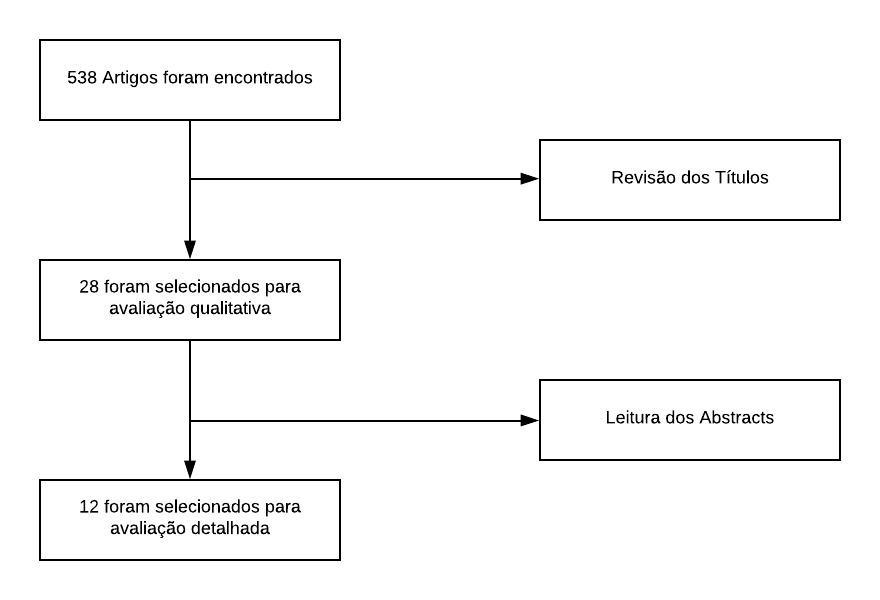
\includegraphics[width = .8\textwidth]{Pictures/revisao_sistematica.jpeg}
    \caption{Fluxograma da Revisão Sistemática}
    \label{fig:revisao_sistematica_fluxograma}
\end{figure}

\section{Resultados e Discussões}
As publicações analisadas têm maior produçnao no ano de 2015, 


\bibliographystyle{sbc}
\bibliography{sbc-template}

\end{document}